\begin{itemize}
	\item Зная конечное распределение ($C_A T_{\odot}^2$) и ограничения на темп аннигиляции  $\Gamma$ из нейтринного сигнала, мы можем ограничить $\sigma_{\chi p}$. 
	\begin{figure}[!h]
		\centering
		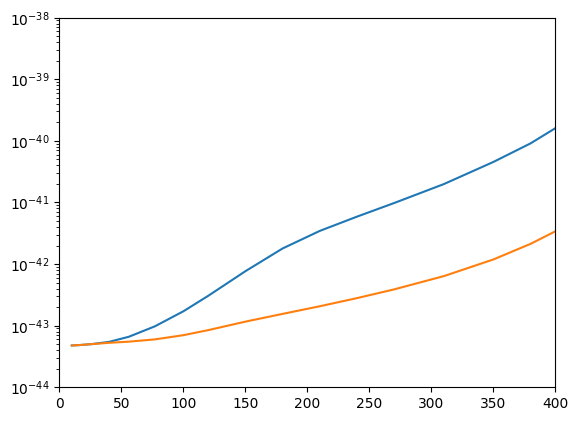
\includegraphics[width=0.55\textwidth]{images/Constrains.png}
		\caption{Ограничения для $m_{\chi} = 100 \, \text{GeV}$ исходя из данных IceCube  на $\Gamma$ в канале $\chi+\chi \to W + W$ (arXiv:1612.05949)} 
	\end{figure}
\end{itemize}
